% Created 2026-07-09 qui 02:53
% Intended LaTeX compiler: lualatex
\documentclass[12pt,a4paper]{article}
\usepackage{fgv-paper}
\usepackage{longtable}
\usepackage{booktabs}
\usepackage{pdflscape}
\usepackage{array}
\usepackage[backend=biber,sorting=nty,giveninits=true]{biblatex}

\usepackage{graphicx}
\author{Gustavo M. Mendes de Tarso}
\date{2026}
\title{Redesenho do fluxo de análise dos benefícios por incapacidade na Perícia Médica Federal: revisão de evidências sobre triagem documental, teleperícia e alocação de capacidade}
\hypersetup{
 pdfauthor={Gustavo M. Mendes de Tarso},
 pdftitle={Redesenho do fluxo de análise dos benefícios por incapacidade na Perícia Médica Federal: revisão de evidências sobre triagem documental, teleperícia e alocação de capacidade},
 pdfkeywords={},
 pdfsubject={},
 pdfcreator={Emacs 28.2 (Org mode 9.5.5)}, 
 pdflang={Brazilian}}
\begin{document}

\maketitle
\tableofcontents


\section{Identificação}
\label{sec:org70bc04f}
\begin{itemize}
\item Perfil: \texttt{relatorio\_prisma\_busca\_orientada\_fgv}.
\item Etapa: busca e triagem pendente.
\item Layout institucional: paper\textsubscript{fgv}.
\item Projeto: prisma\textsubscript{fluxo}\textsubscript{pmf}.
\end{itemize}

\section{Questão e escopo da revisão}
\label{sec:orgf886e1d}
\begin{itemize}
\item Tema: Redesenho baseado em evidências do fluxo de análise dos benefícios por incapacidade na Perícia Médica Federal
\item Recorte: Brasil; organização do fluxo entre análise documental, teleperícia, perícia presencial, capacidade ordinária e mutirões. O ATESTMED é tomado como referência institucional de análise documental, sem restringir a busca à experiência brasileira.
\item Objetivo: Analisar evidências e alternativas para redesenhar o tratamento de requerimentos por incapacidade, combinando análise documental, avaliação remota, perícia presencial, capacidade territorial e critérios auditáveis de alocação.
\item Pergunta de pesquisa: Como estruturar um fluxo de alocação de requerimentos entre análise documental, teleperícia e perícia presencial que reduza o tempo de espera sem comprometer a qualidade decisória, a equidade territorial e o controle?
\item Tipo de estudo: revisão estruturada de evidências para análise e redesenho de política pública
\end{itemize}

\section{Protocolo de busca}
\label{sec:orgf30bade}
\begin{itemize}
\item Estratégia: \texttt{blocos\_tematicos}.
\end{itemize}
\subsection{Blocos e consultas executadas}
\label{sec:orgf5da62b}
\begin{itemize}
\item Benefícios por incapacidade e avaliação médico-pericial: \texttt{disability benefits AND medical assessment}
\item Benefícios por incapacidade e avaliação médico-pericial: \texttt{incapacity benefit AND medical evaluation}
\item Benefícios por incapacidade e avaliação médico-pericial: \texttt{work disability AND medical certification}
\item Análise documental e elegibilidade: \texttt{documentary assessment AND disability}
\item Análise documental e elegibilidade: \texttt{medical certificate AND disability benefits}
\item Análise documental e elegibilidade: \texttt{medical documentation AND work incapacity}
\item Teleperícia e avaliação remota: \texttt{remote medical assessment AND disability}
\item Teleperícia e avaliação remota: \texttt{telemedicine AND disability assessment}
\item Teleperícia e avaliação remota: \texttt{telehealth AND medical certification}
\item Capacidade, filas e alocação de serviços: \texttt{disability benefits AND waiting time}
\item Capacidade, filas e alocação de serviços: \texttt{medical assessment AND service capacity}
\item Capacidade, filas e alocação de serviços: \texttt{case allocation AND disability services}
\item Equidade territorial, qualidade e controle: \texttt{disability assessment AND equity of access}
\item Equidade territorial, qualidade e controle: \texttt{remote assessment AND quality assurance}
\item Equidade territorial, qualidade e controle: \texttt{medical certification AND audit}
\item Palavras-chave: benefícios por incapacidade; disability benefits assessment; análise documental de incapacidade; documentary review disability claims; teleperícia; telemedicine disability evaluation; perícia médica presencial; triagem de requerimentos por incapacidade; work capacity assessment; gestão de filas em saúde; equidade territorial no acesso; auditabilidade de decisões administrativas
\item Idiomas: português; inglês; espanhol
\item Bases selecionadas: Crossref; OpenAlex; Semantic Scholar; Scopus; Web of Science; PubMed/NCBI; Europe PMC; SciELO; CORE
\end{itemize}

\subsection{Critérios de inclusão}
\label{sec:orgd8e3f14}
\begin{itemize}
\item Estudos que analisem benefícios por incapacidade, afastamento por doença, seguro por incapacidade, certificação médica ou avaliação médico-pericial.
\item Estudos que abordem triagem documental, elegibilidade, análise de documentos médicos, validação de atestados ou processos de decisão sobre incapacidade.
\item Estudos que examinem teleperícia, telemedicina aplicada à avaliação, avaliação médica remota, videoperícia ou modalidades híbridas de avaliação.
\item Estudos que analisem capacidade operacional, filas, tempo de espera, produtividade, priorização de casos, alocação de profissionais ou gestão de demanda em serviços periciais ou sistemas de benefícios.
\item Estudos que discutam acesso territorial, equidade, barreiras geográficas, inclusão de populações remotas ou desigualdades de acesso à avaliação médico-pericial.
\item Estudos que tratem de qualidade decisória, confiabilidade, auditoria, controle, integridade, prevenção de fraude, revisão de decisões ou riscos associados à avaliação remota ou documental.
\item Estudos empíricos, avaliações de política pública, estudos de caso institucionais, revisões sistemáticas, revisões de escopo ou relatórios técnicos com evidência útil para a pergunta de pesquisa.
\item Publicações em português, inglês ou espanhol.
\end{itemize}

\subsection{Critérios de exclusão}
\label{sec:org71b200c}
\begin{itemize}
\item Telemedicina exclusivamente assistencial, sem relação substantiva com avaliação de incapacidade, certificação, elegibilidade, triagem ou gestão de fluxos.
\item Estudos clínicos que não contribuam para compreender processos de avaliação médico-pericial, decisão administrativa, capacidade, acesso, qualidade ou controle.
\item Textos sem relação substantiva com a pergunta de pesquisa ou com ao menos um eixo da matriz analítica.
\item Editorial, comentário, notícia, apresentação, resumo de congresso ou opinião sem análise, dados, revisão ou contribuição institucional verificável.
\item Duplicidades entre bases ou consultas.
\item Registros sem título, resumo ou metadados suficientes para triagem humana.
\item Publicações em idioma diferente de português, inglês ou espanhol quando não houver informação suficiente para avaliação confiável.
\end{itemize}

\section{Registro por fonte}
\label{sec:org3c8b529}
\begin{center}
\begin{tabular}{lrl}
Base & Registros recuperados & Situação\\
\hline
Crossref & 300 & ok\\
OpenAlex & 300 & ok\\
Semantic Scholar & 200 & parcial\\
Scopus & 15 & ok\\
Web of Science & 0 & não executada: credencial ausente\\
PubMed/NCBI & 289 & ok\\
Europe PMC & 300 & ok\\
SciELO & 0 & bloqueada por anti-automação\\
CORE & 255 & parcial\\
\end{tabular}
\end{center}

\section{Fluxo de seleção}
\label{sec:org4f23a6e}

\begin{figure}[htbp]
\centering
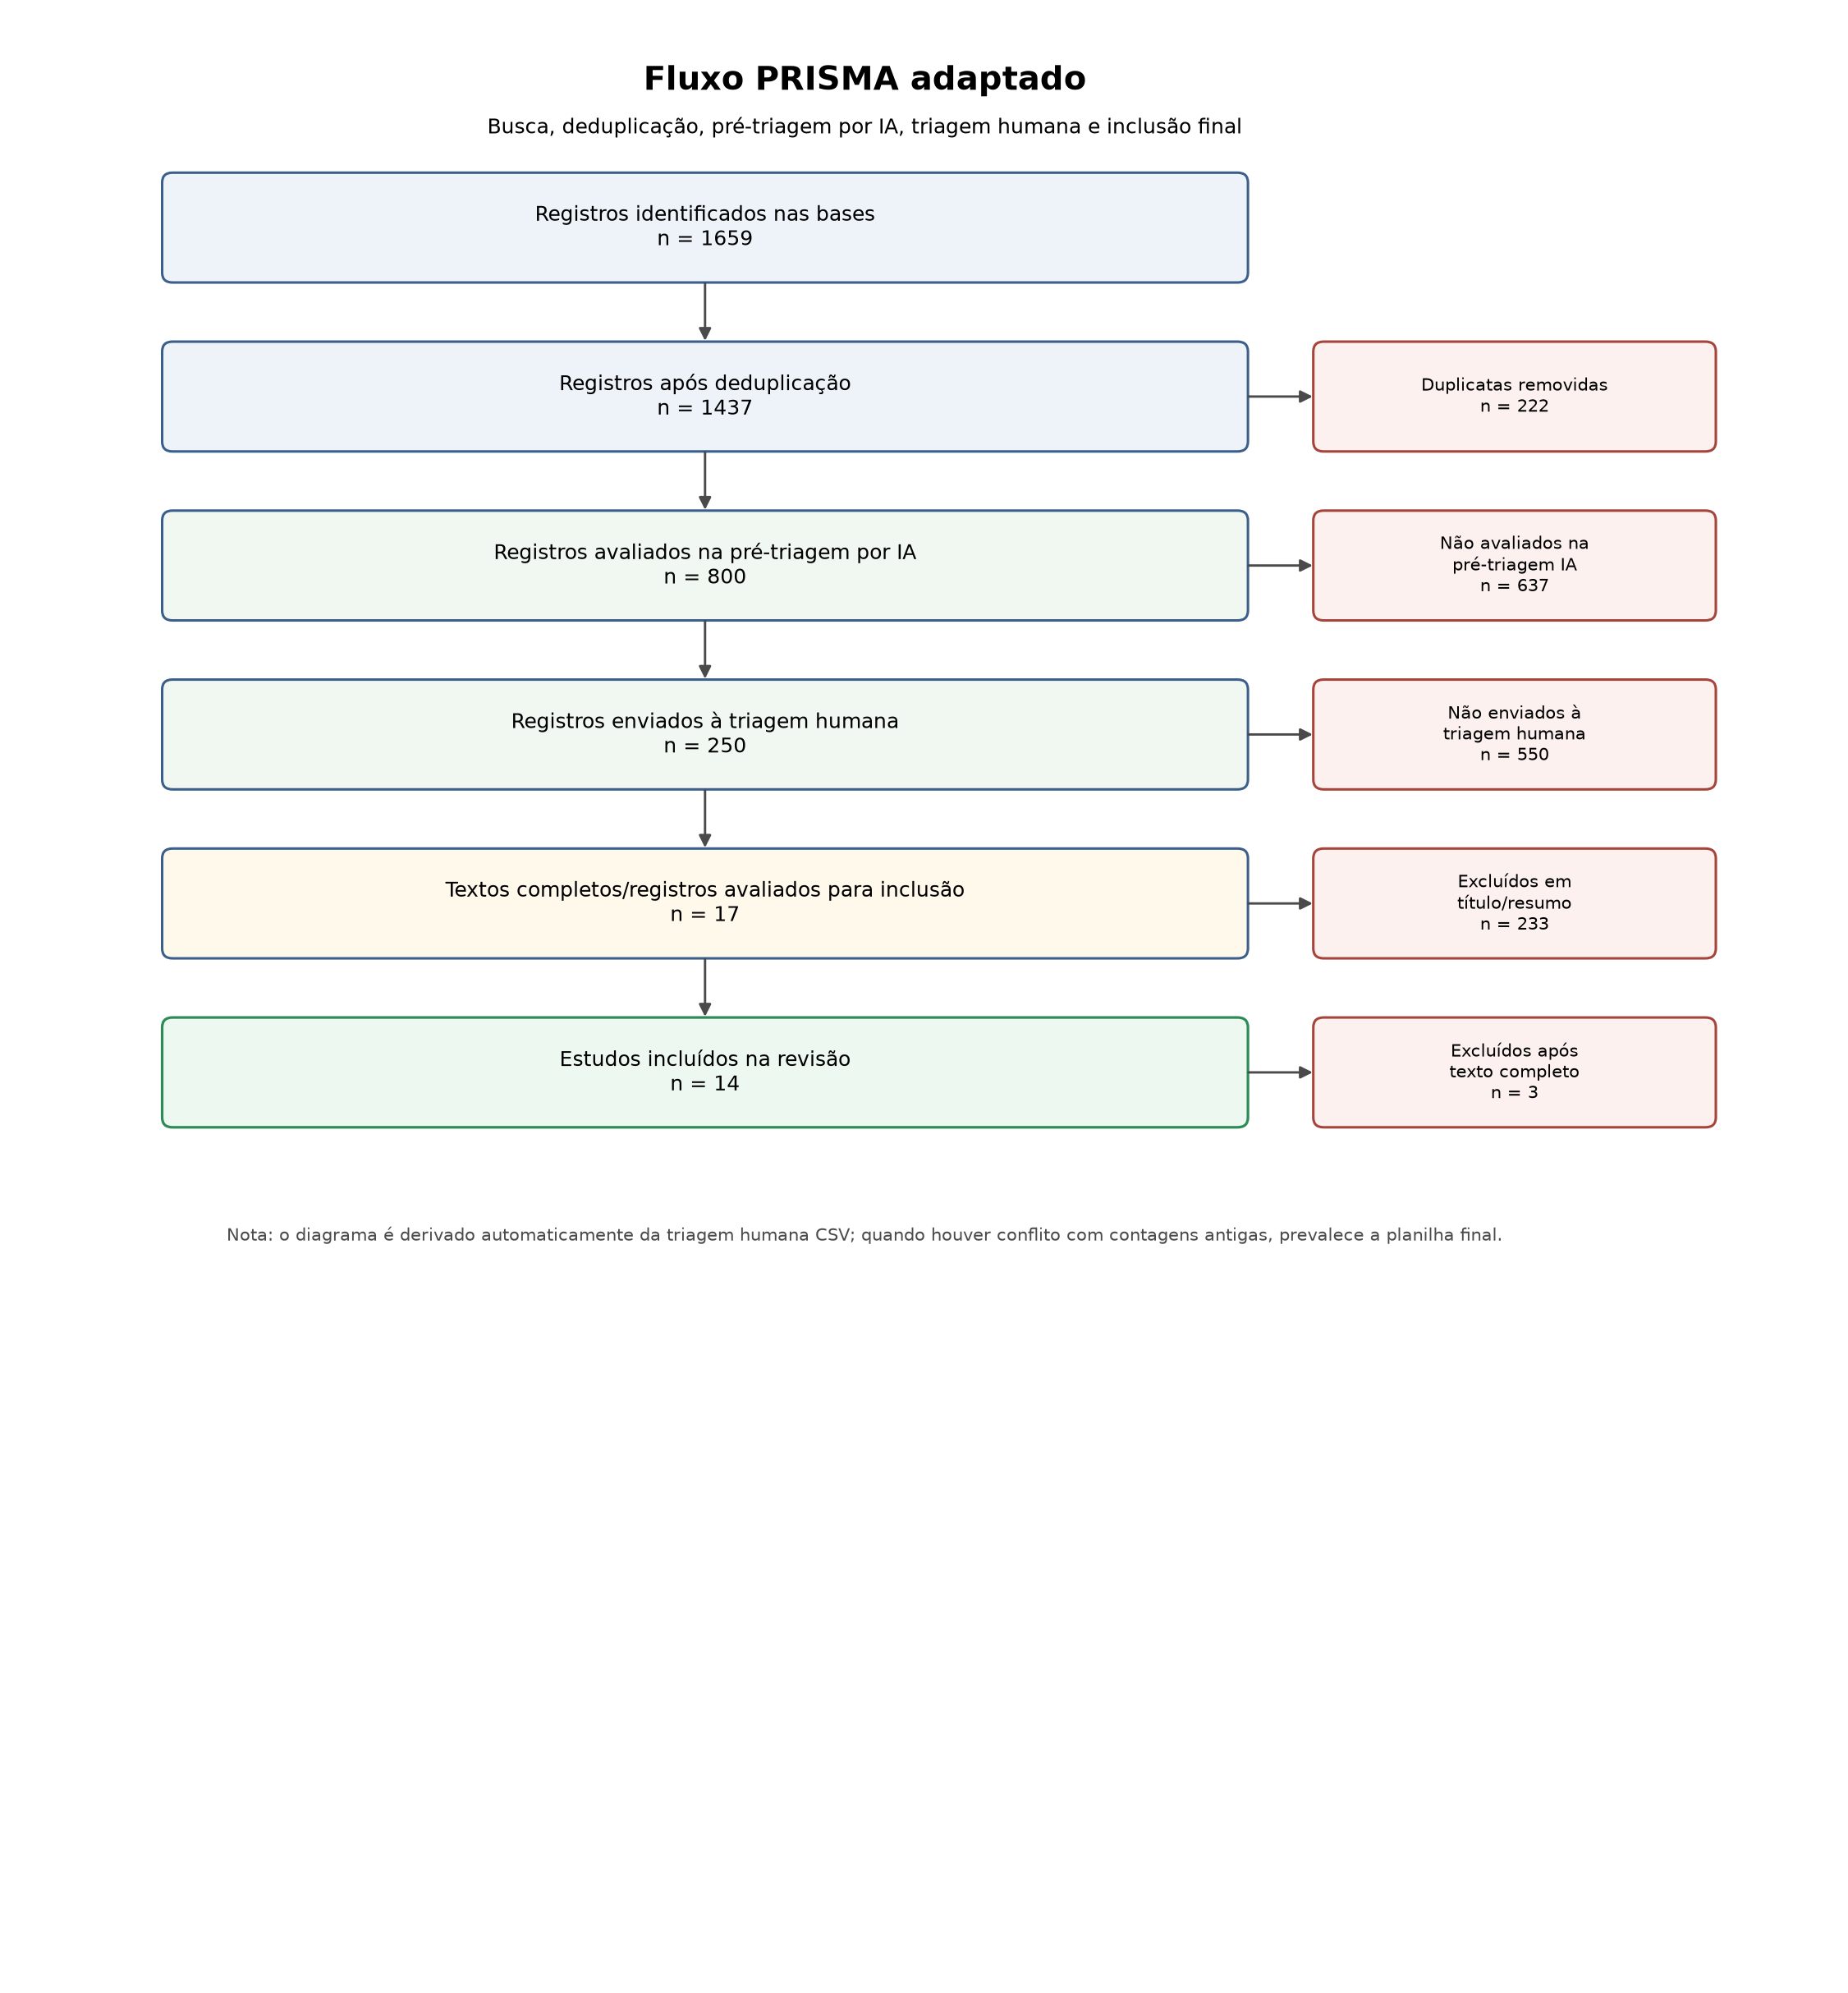
\includegraphics[width=0.95\textwidth]{relatorio_prisma_prisma_fluxo_pmf.diagrama_prisma.png}
\caption{Diagrama PRISMA adaptado ao fluxo de busca, pré-triagem por IA e triagem humana.}
\end{figure}

\begin{center}
\begin{tabular}{lr}
Etapa & Quantidade\\
\hline
registros identificados & 1659\\
duplicatas removidas & 222\\
registros apos deduplicacao & 1437\\
registros pre triagem ia avaliados & 1437\\
registros enviados para triagem & 250\\
triagem titulo resumo concluida & 250\\
registros excluidos titulo resumo & 231\\
textos completos avaliados & 19\\
textos completos excluidos & 2\\
estudos incluidos & 17\\
registros na planilha & 250\\
\end{tabular}
\end{center}

A figura apresenta o funil de seleção da revisão. As contagens finais de triagem humana são derivadas do arquivo \texttt{triagem\_humana.csv}; quando contagens intermediárias antigas entram em conflito com a planilha final, prevalece a reconciliação pela decisão humana final.

\section{Situação da triagem}
\label{sec:org316ed90}
A busca foi concluída, mas a inclusão e a exclusão de estudos permanecem pendentes de decisão humana na planilha de triagem.
\begin{itemize}
\item A planilha foi ordenada por pré-triagem assistida por IA antes do limite inicial de registros.
\item A recomendação e a justificativa da IA servem apenas para priorização; elas não substituem a decisão humana.
\item Planilha de triagem: \texttt{/home/gustavodetarso/Documentos/mppg/software/academic\_pipeline\_rc10\_7\_conformidade/app\_bundle/projetos/prisma\_fluxo\_pmf/output\_pesquisa/relatorio\_prisma\_prisma\_fluxo\_pmf/relatorio\_prisma\_prisma\_fluxo\_pmf.triagem\_titulo\_resumo.xlsx}
\item Após preencher a planilha, importe-a com \texttt{-{}-prisma-importar-triagem}. O pipeline então produzirá a versão final deste relatório no mesmo layout e com a mesma engine PDF configurada no TOML.
\end{itemize}

\section{Nota metodológica}
\label{sec:orgbc929dc}
Este documento registra a estratégia de descoberta e a situação da triagem. Ele não apresenta a busca como revisão concluída nem substitui a avaliação humana dos títulos, resumos e textos completos.
\end{document}